\documentclass[../main.tex]{subfiles}

\begin{document}
Ovde je, na slici \ref{fig:igraonice}, prikazana sekcija koja sadrži aktuelne pakete usluga za igraonice (dečije i PS). Ovo je jedna od sekcija kojoj može pristupiti samo registrovan i prijavljen korisnik (odnosno, klijent). Klijent bira paket o kome želi da dobije dodatne informacije klikom na vezu ``Prikaži više...``, koja vodi ka posebnoj stranici sa detaljnim opisom izabranog paketa i cenom. Ukoliko klijent, nakon usvajanja ovih informacija, i dalje želi taj paket, klikom na dugme ``Kupi paket`` započinje kupovinu. Naredni korak podrazumeva popunjavanje formulara, koji se prikazuje korisniku nakon sto je kliknuo na pomenuto dugme. U formularu navodi svoje osnovne informacije i bira program. Nakon što klijent pristane da nastavi dalje, prelazi se na formular za plaćanje, koji je detaljnije opisan u sekciji-------------------.

\begin{figure}[!ht]
\begin{center}
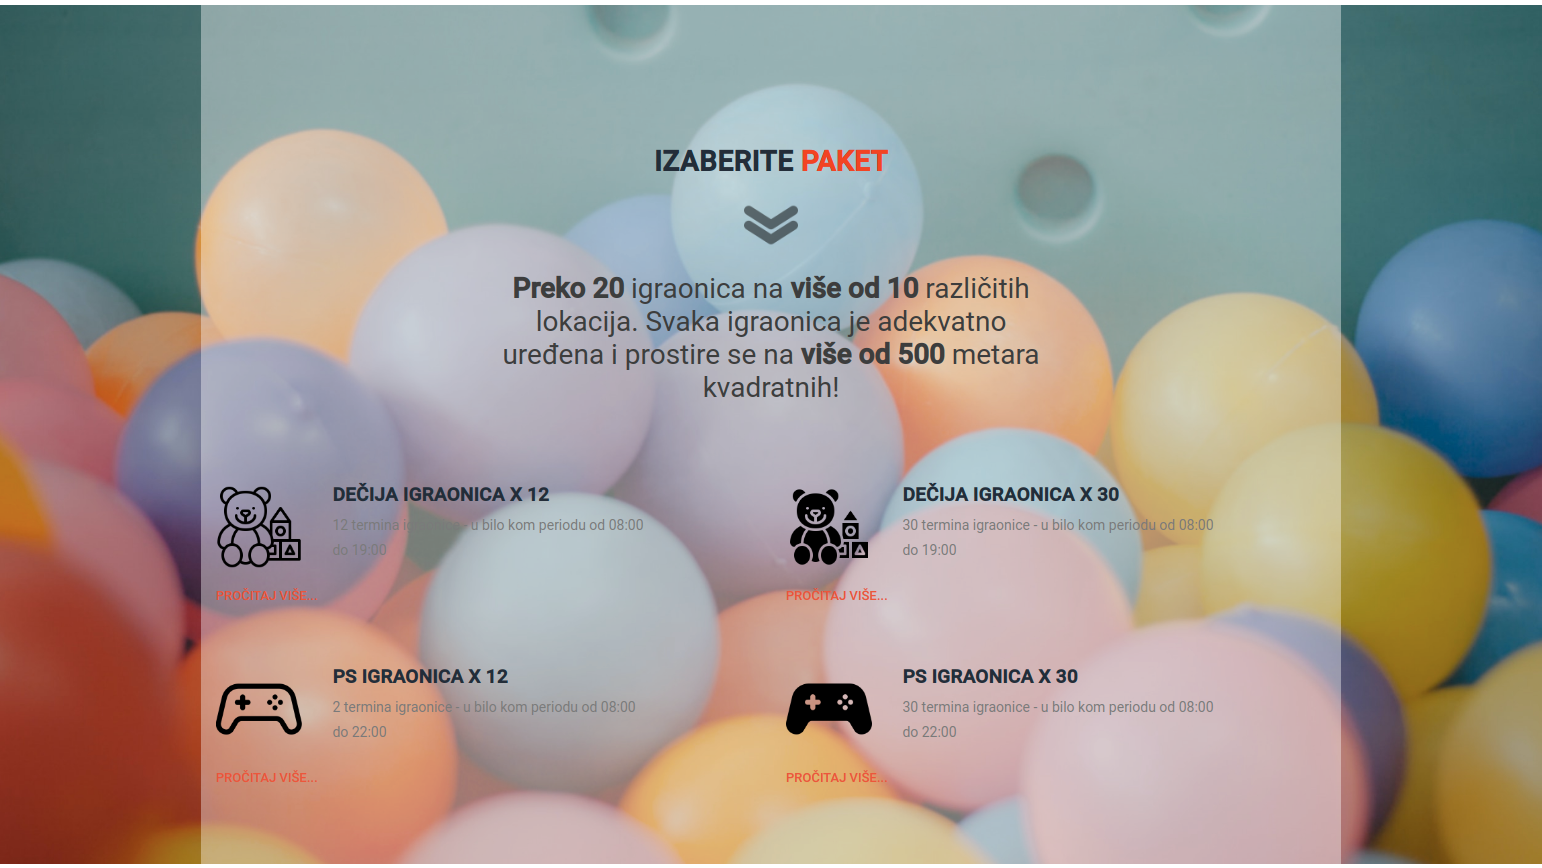
\includegraphics[scale=0.22]{sections/korisnicki_interfejs/screenshots/ponude_igraonice.png}
\end{center}
\caption{Paketi usluga igraonica}
\label{fig:igraonice}
\end{figure}

U nastavku je prikazan izgled stranica koje sadrže opise paketa i cene. Na slici (\ref{fig:decijax12} prva) je prikazana stranica u kojoj je dat opis paketa ``DEČIJA IGRAONICA x 12``, dok je na slici (\ref{fig:decijax12} treća) stranica koja sadrži opis paketa ``PS IGRAONICA x 12``. Slede slike (\ref{fig:decijax12} druga) i (\ref{fig:decijax12} četvrta), na kojima su prikazane stranice u kojima su opisani paketi ``DEČIJA IGRAONICA x 30`` i ``PS IGRAONICA x 30`` redom.

\begin{figure}[!ht]
\begin{center}
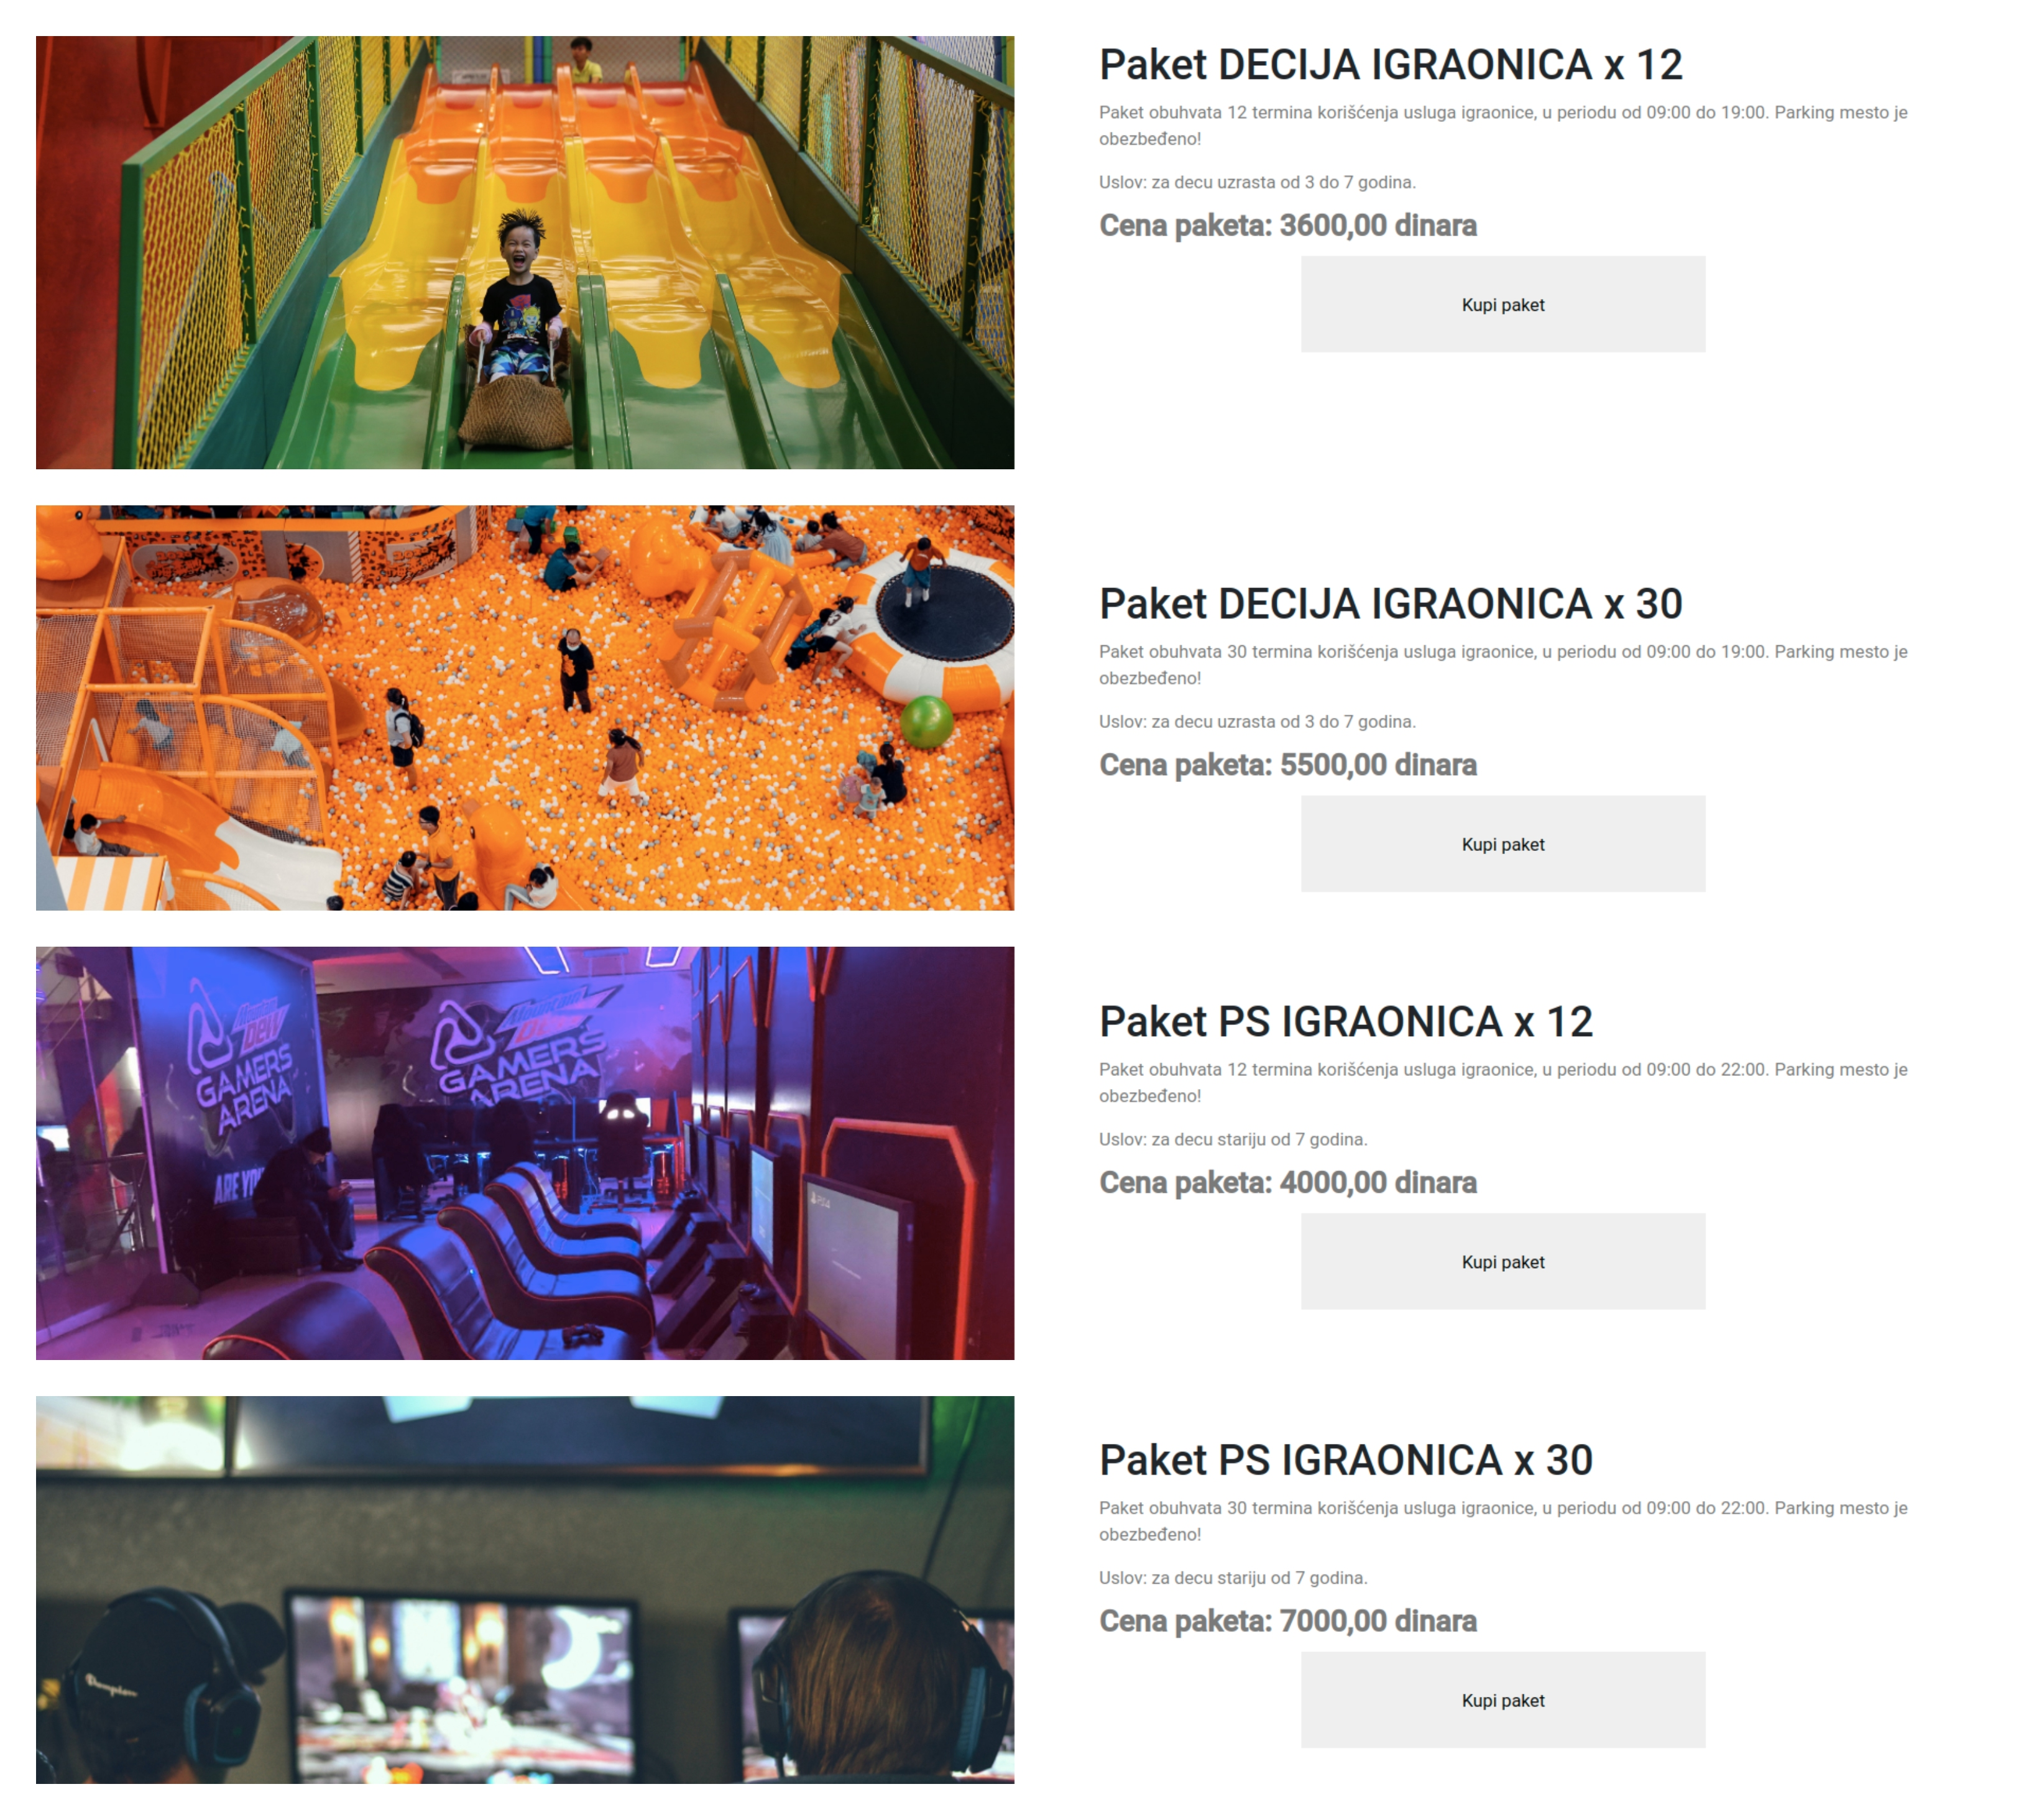
\includegraphics[scale=0.20]{sections/korisnicki_interfejs/screenshots/paketiIgraonica.jpg}
\end{center}
\caption{Odozgo na dole: Opis paketa ``DEČIJA IGRAONICA x 12``, Opis paketa ``DEČIJA IGRAONICA x 30``, Opis paketa ``PS IGRAONICA x 12``, Opis paketa ``PS IGRAONICA x 30``}
\label{fig:decijax12}
\end{figure}

\end{document}